\documentclass[a4paper, oneside]{article} 

\usepackage[a4paper, left=17mm, right=17mm, top=25mm, bottom=25mm]{geometry}
\usepackage{amsfonts}
\usepackage{amsmath}
\usepackage{graphicx}
\usepackage{multicol}
\setlength{\columnsep}{7mm}
\setlength{\textwidth}{176mm}
\usepackage{mathtools}
\usepackage{dsfont}
\usepackage{xparse}
\usepackage{caption}

\usepackage{listings}
\usepackage{xcolor}
\lstset{
  language=Python,
  basicstyle=\ttfamily\scriptsize,
  backgroundcolor=\color{gray!5},
  frame=single,
  rulecolor=\color{black!20},
  breaklines=true,
  breakatwhitespace=true,
  captionpos=b,
  tabsize=4,
  keepspaces=true,
  showspaces=false,
  showstringspaces=false,
  showtabs=false,
  numbers=none,
  xleftmargin=1pt,
  framexleftmargin=1pt,
  aboveskip=1em,
  belowskip=1em
}


\newcommand{\code}[1]{\texttt{#1}}

\title{A FEniCSx toolbox for level set-based shape and topology optimization supporting parallel computing}
\author{
	Josu\'{e} D. D\'{i}az-Avalos\thanks{Email: \texttt{josue.diazavalos@uni-due.de}} \qquad
	Antoine Laurain\thanks{Email: \texttt{antoine.laurain@uni-due.de}} \\
	\\
	Fakultät für Mathematik, Universität Duisburg-Essen
}
\date{\today}

\begin{document}

\maketitle

\begin{abstract}
We present a toolbox for shape and topology optimization using the software package FEniCSx.
The optimization is based on the distributed shape derivative.
The numerical shape modeling uses a standard level set method.
The implementation supports parallel computing in two different modes.
On one hand, the built-in features of FEniCSx for parallelizing the mesh are used.
On the other hand, we also implement a parallelization of the source terms in the underlying partial differential equations. The user can then conveniently use a combination of the two modes for parallel computing.
\end{abstract}

\begin{multicols}{2}


\section{Introduction}
Here we emphasize the following points:
\begin{itemize}
    \item Literature review: there are many papers to cite. Many recents eductional codes available. \cite{Wegert2025}
\item The paper is a continuation of \cite{MR3843884}.
\item The goal is to provide a toolbox that is easy to use and allows to test some shape optimization problems in a fast way. Suited for students and practitioners. The main work for someone using the toolbox is to write an appropriate model (geometry and PDE) and compute $S_1,S_0$.
\item There are many eductional papers and implementations for structural optimization and topology optimization, but they usually focus on the SIMP method, or an approximation of the level set method (clarify). Here we provide an implementation based on the distributed shape derivative. 
\item On one hand, the  distributed shape derivative has practical advantages: accuracy and ease of implementation. From the educational point of view, it is a way to learn about shape sensitivity analysis.
\item Unlike similar papers on the topic, we focus here mainly on inverse problems, which benefit greatly from the parralelization of the sources.
\item We also want to explain how the parralelization works, in a pedagogical way.
\end{itemize}    

General problem
\begin{equation} \label{eq:problem}
	\min_{\Omega\subset\mathcal{D}} J(\Omega)
	\quad \text{subject to} \quad C(\Omega) = \boldsymbol{1}
\end{equation}
$J$ is the cost functional, $C$ is the vector-valued constraint function
%%%%%%%%%%%%%%%%%%%%%%%
\section{Shape derivatives}
%%%%%%%%%%%%%%%%%%%%%%%
This will be similar to \cite[Section 2]{MR3843884},
recalling definitions of distributed and boundary expression of shape derivative.


Notations. Let $\mathcal{D}\subset\mathds{R}^d$ be open bounded domain with boundary
$\Gamma = \partial \mathcal{D}$. Let $n$ denote the outward unit normal vector to $\Gamma$.
Let $I$ denote the $d$-dimensional identity matrix. $\left|\cdot\right|_{\infty}$ denotes the infinity norm.
\begin{equation}
	dJ(\Omega) \theta = \int_{\mathcal{D}} S_0^J \cdot \theta + S_1^J : D\theta 
\end{equation}
\begin{equation}
	dC(\Omega) \theta = \int_{\mathcal{D}} S_0^C \cdot \theta + S_1^C : D\theta 
\end{equation}
%%%%%%%%%%%%%%%%%%%%%%%
\section{Shape derivative for a model problem}
%%%%%%%%%%%%%%%%%%%%%%%

Here one could show the calculation of the distributed shape derivative for a model problem. 
One should choose a different problem from \cite[Section 3]{MR3843884},
for instance the inverse problem in elasticity. One could add another
subsection with another model problem, for instance heat equation,
where one would just show the result with the tensors $S_1,S_0$.

\textbf{Inverse Problem in Linear Elasticity.}
Let $\Gamma_0$, $\Gamma_1$ subsets of $\Gamma$. 
The stress and symmetric strain tensors are given by
\begin{equation*}
	\sigma(w)=2\mu\,\epsilon(w)+\lambda(\nabla\cdot w)I,\quad  \epsilon(w)=\frac{Dw+{Dw}^{\top}}{2}.
\end{equation*}
Let $H_{\Gamma_0}(\mathcal{D})^d$ be the space of functions
\begin{equation*}
	H_{\Gamma_0}(\mathcal{D})^d\coloneqq\left\{ u\in H(\mathcal{D})^{d}\mid u|_{\Gamma_0}=\boldsymbol{0}\right\} 
\end{equation*}
The optimization problem reads:
\begin{equation} \label{eq:InvProb}
	\min_{\Omega \subset \mathcal{D}}
	\frac{\alpha}{2}\int_{\mathcal{D}}\left|u-v\right|^{2} + 
	\frac{\beta}{2}\int_{\Gamma_{1}}\left|u-v\right|^{2}
\end{equation}
where $u$ and $v$ are the solutions to
\begin{equation} \label{eq:f-prob}
	\begin{array}{rcl}
    -\mathrm{div} A_{\Omega} \sigma(u) = 0 & \text{in} & \mathcal{D} \\
                                u = 0 & \text{on} & \Gamma_{0} \\
                 A_{\Omega} \sigma(u)n = f & \text{on} & \Gamma_{1} \\
                 A_{\Omega} \sigma(u)n = 0 & \text{on} & \Gamma \setminus (\Gamma_{1} \cup \Gamma_{1})                     
	\end{array}	
\end{equation}
and
\begin{equation} \label{eq:g-prob}
	\begin{array}{rcl}
    -\mathrm{div} A_{\Omega} \sigma(v) = 0 & \text{in} & \mathcal{D} \\
                                v = 0 & \text{on} & \Gamma_{0} \\
                                v = g & \text{on} & \Gamma_{1} \\
            A_{\Omega} \sigma(v)n = 0 & \text{on} & \Gamma \setminus (\Gamma_{1} \cup \Gamma_{1})    
	\end{array}
\end{equation}
respectively. The weak formulation of \eqref{eq:f-prob} reads:
Find $u \in  H^1_{\Gamma_0}(\mathcal{D})^d$ such that
\begin{equation} \label{eq:w-f}
	\int_{\mathcal{D}} A_{\Omega}\sigma(u):\epsilon(w) =
	\int_{\Gamma_1} f \cdot w
	\quad
	\forall \, w \in  H^1_{\Gamma_0}(\mathcal{D})^d
\end{equation}
By extending $g$ to the whole domain,
the weak formulation of \eqref{eq:g-prob}
is written in such a way that we seek a solution
in $H^1_{\Gamma_0}(\mathcal{D})^d$:
Find $v \in  H^1_{\Gamma_0}(\mathcal{D})^d$ such that
\begin{equation} \label{eq:w-g}
	\int_{\mathcal{D}} A_{\Omega}\sigma(v + g):\epsilon(w) = 0
	\quad
	\forall \, w \in  H^1_{\Gamma_0}(\mathcal{D})^d
\end{equation}
From \eqref{eq:w-f} and \eqref{eq:w-g},
the Lagrangian functional for \eqref{eq:InvProb}
is defined by
\begin{equation} \label{eq:elastic_lag}
	\mathcal{L}(\Omega,\varphi, \psi, \rho, \varrho) =
	\mathcal{L}_{\mathrm{cost}} +
	\mathcal{L}_{\mathrm{state}} +
	\mathcal{L}_{\mathrm{adjoint}}
\end{equation}
\begin{align*}
	\mathcal{L}_{\mathrm{cost}}    &= \frac{\alpha}{2}\int_{\mathcal{D}} \left|\varphi-\psi - g\right|^{2} + \frac{\beta}{2}\int_{\Gamma_{1}} \left|\varphi - g \right|^{2} \\
	\mathcal{L}_{\mathrm{state}}   &= \int_{\mathcal{D}} A_{\Omega} \sigma(\varphi) : \epsilon(\rho) - \int_{\Gamma_{1}} f \cdot \rho \\
	\mathcal{L}_{\mathrm{adjoint}} &= \int_{\mathcal{D}} A_{\Omega} \sigma(\psi + g) : \epsilon(\varrho)
\end{align*}
Deriving $\mathcal{L}$, we obtain the adjoint equations
\begin{align*} \label{eq:f-adj}
\int_{\mathcal{D}} A_{\Omega}\sigma(p):\epsilon(r) & = -\alpha \int_{\mathcal{D}} (u-v-g) \cdot r \\
&\quad -\beta \int_{\Gamma_1} (u - g) \cdot r \quad
\forall \, r \in  H^1_{\Gamma_0}(\mathcal{D})^d	\nonumber
\end{align*}
and
\begin{equation*} \label{eq:g-adj}
	\int_{\mathcal{D}} A_{\Omega}\sigma(q):\epsilon(r) =
	\alpha \int_{\mathcal{D}} (u-v-g) \cdot r \quad \forall \, r \in  H^1_0(\mathcal{D})^d.
\end{equation*}
In order to obtain the shape derivative of $J$, we define
\begin{align*}
	& \mathcal{G}(t,\varphi,\psi,\rho,\varrho) \coloneqq\\
	& \mathcal{L}\left(\Omega_{t},\varphi\circ T_{t}^{-1},\psi\circ T_{t}^{-1},\rho\circ T_{t}^{-1},\varrho\circ T_{t}^{-1}\right)
\end{align*}
Applying the change of variable $x \mapsto T_t(x)$,
\begin{equation*}
	\mathcal{G}(t,\varphi,\psi,\rho,\varrho) =
	\mathcal{G}_{\mathrm{cost}} +
	\mathcal{G}_{\mathrm{state}} +
	\mathcal{G}_{\mathrm{adjoint}}
\end{equation*}
\begin{align*}
	\mathcal{G}_{\mathrm{cost}}    &= \frac{\alpha}{2}\int_{\mathcal{D}}\left|\phi-\varphi-g\circ T_{t}\right|^{2}\xi(t)+\frac{\beta}{2}\int_{\Gamma_{1}}\left|\phi-g\right|^{2} \\
	\mathcal{G}_{\mathrm{state}}   &= \int_{\mathcal{D}}A_{\Omega}E(t,\phi):E(t,\rho)\xi(t)-\int_{\Gamma_{1}}f\cdot\rho \\
	\mathcal{G}_{\mathrm{adjoint}} &= \int_{\mathcal{D}}A_{\Omega}E(t,\varphi + g\circ T_{t}):E(t,\varrho)\xi(t)
\end{align*}
Since
\begin{equation}
	dJ(\Omega; \theta) = \partial_{t}\mathcal{G}(0, u, v, p, q),
\end{equation}
we derivate $\mathcal{G}$ with respect to $t$ and
evaluate it at $(0,u,v,p,q)$ to obtain
\begin{equation}
	dJ(\Omega; \theta) = \int_{\mathcal{D}} S_0^J \cdot \theta + S_1^J : D\theta 
\end{equation}
with $S_0^J$ and $S_1^J$ given by
\begin{equation*}
	S^{J}_{0} = -\alpha{Dg}^{\top}(u - v - g) +
	A_{\Omega}\sum_{i,j=1}^{d}{\sigma (q)}_{i,j}\nabla(\epsilon(g)_{i,j})
\end{equation*}
and
\begin{align*}
	S^{J}_{1} & = \frac{\alpha}{2}{|u-v-g|}^2 I\\
			  & \quad + \left(A_{\Omega}\sigma(u):\epsilon(p) + A_{\Omega}\sigma(v+g):\epsilon(q)\right)I\\
			  & \quad + A_{\Omega} \left({Du}^{\top}\sigma(p) + {Dp}^{\top}\sigma(u)\right)\\
			  & \quad + A_{\Omega} \left({Dv}^{\top}\sigma(q) + {Dq}^{\top}\sigma(v+g)\right),
\end{align*}
respectively.
In addition, it is necessary to choose a bilinear form
in order to find the velocity field to compute the level set function.
We choose $B:H^1(\mathcal{D})^d \times H^1(\mathcal{D})^d \rightarrow \mathds{R}$
defined by
\begin{equation}
	B(\theta, \xi) = \int_{\mathcal{D}} {10}^{-1}\theta \cdot \xi + D\theta : D\xi 
\end{equation}
Find $\theta \in H^1(\mathcal{D})^d$ such that
\begin{equation}
	B(\theta, \xi) = - dJ(\Omega; \xi) \quad \forall\, \xi\in H^1(\mathcal{D})^d.
\end{equation}
%%%%%%%%%%%%%%%%%%%%%%%
\section{Numerical implementation}
%%%%%%%%%%%%%%%%%%%%%%%

%%%%%%%%%%%%%%%%%%%%%%%
\subsection{Toolbox structure}
%%%%%%%%%%%%%%%%%%%%%%%

Here explain how the toolbox is organized.
The folder ``Models'' will contain the files for each model. One for inverse problem in elasticity, one for heat equation, etc ... For each model, what changes is the PDEs, the geometric configuration such as boundary conditions and domain, and the tensors $S_1,S_0$.

The folder ``Shape'' (?) will contain the files for the shape optimization, this includes in particular the file for the level set method.

\subsection{Model construction}
We start by creating a subclass of \code{Model} class
with the following necessary attributes and methods:
\begin{lstlisting}
from distributed import Model

class MyModel(Model):

    def __init__(self, dim, domain, space, path):

        self.dim = dim
        self.domain = domain
        self.space = space
        self.path = path

	def pde(self, phi):
		pass
	
	def adjoint(self, phi, U):
		pass

	def cost(self, phi, U):
		pass
	
    def constraint(self, phi, U):
		pass

	def derivative(self, phi, U, P):
	 	pass
	
	def bilinear_form(self, th, xi):
		pass
\end{lstlisting}
The attributes \code{dim}, \code{domain}, \code{space}, and \code{path}
are the dimension of the problem domain $d$, the mesh that represents the domain $\Omega$,
the space of functions for the problem solutions, and the test path where the results will be saved, respectively. 

The \code{pde} method models the partial differential equations of the problem.
It must return a list with elements of the form \code{(wk, bc)},
where \code{wk} is the weak formulation of the equations
and \code{bc} is a list with the Dirichlet boundary conditions.
The \code{adjoint} method model the adjoint equations of the problem.
It must return a list of similar struct that \code{pde}. 
The \code{cost} method must return the cost functional $J(\Omega)$.
The \code{constraint} method must return a list with the components of $C(\Omega)$.
The \code{derivative} method must return two tuples,
each one with the derivative components $S_0$ and $S_1$, respectively,
corresponding to the cost functional and the constraints.
Finally, the \code{bilinear\_form} method must return
the chosen bilinear form $B(\theta, \xi)$.

All the content of this class must be written exclusively using
UFL and native Python functions. Details of the input and outputs of these methods
can be view in the documentation of the \code{Model} class. 


%%%%%%%%%%%%%%%%%%%%%%%
\subsection{Parallelization}
%%%%%%%%%%%%%%%%%%%%%%%

Here we explain the two modes of parallelization, the mesh and the sources,
and how the user can play with that. Explain the splitting and the colors.

Cite some parts of the codes to explain that.

Data parallelism, Task parallelism, and Mix parallelism (a mix of previous ones)  

%%%%%%%%%%%%%%%%%%%%%%%
\subsection{Augmented Lagrangian}
%%%%%%%%%%%%%%%%%%%%%%%

Here explain how the augmented Lagrangian works for volume constraints 

\begin{equation} \label{eq:lagrangian}
\begin{aligned}
	L(\Omega, z, \lambda, \mu) =\,
	& J(\Omega) + \langle \lambda, C(\Omega) -  \boldsymbol{1} \rangle + \langle \mu, z \rangle \\
	& + \frac{\alpha}{2} \Vert z \Vert^2 + \frac{\beta}{2} \Vert \lambda - \mu \Vert^2
\end{aligned}
\end{equation}

$S_0$ and $S_1$ in \eqref{eq:velocity} given by
\[
	S_0 = S_0^{J} + \lambda^{i} S_0^{C}, \quad S_1 = S_1^{J} + \lambda^{i} S_1^{C} 
\]
where $\lambda^{i}$ is updated following the algorithm
proposed in \cite{MR4589221}: given 
$r\in(0,1)$,
$\alpha\in(1,\infty)$, $\beta\in(0,1)$, 
$\delta^{0}\in(0,1]$, and 
$(z^{0},\lambda^{0},\mu^{0})$
do
\begin{equation} \label{eq:lag_method}
	\begin{aligned}
		\mu^{i+1} & = \mu^{i}+\delta^{i}(\lambda^{i}-\mu^{i})(\left\Vert \lambda^{i}-\mu^{i} \right\Vert^{2} + 1)^{-1}\\
		\lambda^{i+1} & = \mu^{i+1} + \alpha (1+\alpha \beta)^{-1}(C(\Omega^{i+1})- \boldsymbol{1})\\
		z^{i+1} & = \alpha^{-1}(\lambda^{i+1}-\mu^{i+1})\\
		\delta^{i+1} & =r\delta^{i}
	\end{aligned}
\end{equation}
for $i=0,1,2,\dots$. Recall that $\Omega^{i+1}$ is obtained in (?).
For all tests we used
$r = 0.999$, $\delta^{0} = 0.5$,
$\alpha = 2000$, $\beta = 0.5$,
$z^{0} = 0$, $\lambda^{0} = 0$, and $\lambda^{0} = 0$.


%%%%%%%%%%%%%%%%%%%%%%%%%%%%%
\subsection{Velocity}
%%%%%%%%%%%%%%%%%%%%%%%%%%%%%
The velocity $\theta$ is obtained by solving the following weak formulation:
Find $\theta\in\mathbb{H}$ such that
\begin{equation} \label{eq:velocity}
	B (\theta, \xi) =
	- \int_{\mathcal{D}} S_0\cdot\xi + S_1 : D\xi \quad\forall \; \xi \in \mathbb{H}
\end{equation}
with $\mathbb{H} = H^1(\mathcal{D})^d$ or $\mathbb{H} = H_0^1(\mathcal{D})^d$.
The bilinear form $B$ must be provided as a UFL expression
in the method \code{bilinear\_form} of the model class.
This method must return \eqref{eq:velocity}, and
either \code{False} (if $\mathbb{H} = H^1(\mathcal{D})^d$)
or \code{True} (if $\mathbb{H} = H_0^1(\mathcal{D})^d$).
The \code{Velocity} class sets up and solve \eqref{eq:velocity}.

If $\mathbb{H} = H^1(\mathcal{D})^d$, consider in $B$
a term of the form
$$
{10}^{5}
$$
in order to have $\theta\cdot n = 0$ (almost zero) on the boundary.

%%%%%%%%%%%%%%%%%%%%%%%%%%%%%
\subsection{Level set method}
%%%%%%%%%%%%%%%%%%%%%%%%%%%%%

Explain how the level set method is implemented, cite the code.
We solve the diffusion-transport problem
\begin{equation} \label{eq:transport}
\begin{aligned}
\partial_t \phi+\theta\cdot\nabla\phi - h^2\nabla^2\varphi &= 0 && x\in \mathcal{D},\, t>0, \\
										 \partial_{n} \phi &= 0 && x\in \partial\mathcal{D},\, t>0, \\
												\phi(0, x) &= \phi^{i}(x) && x\in \mathcal{D},
\end{aligned}
\end{equation}
We choose $\phi^{i+1}(x) = \phi(T,x)$.
The Petrov-Galerkin method \cite{MR1640142} with the Crank-Nicolson method yields
\begin{align} \label{eq:weak_transport}
	& \int_{\mathcal{D}} \phi(t+\Delta t,\cdot)\hat{\psi} + \Delta t \, \mathcal{F}(\phi(t+\Delta t,\cdot), \hat{\psi}) = \nonumber \\
	& \int_{\mathcal{D}} \phi(t,\cdot) \hat{\psi} - \Delta t \, \mathcal{F}(\phi(t,\cdot), \hat{\psi})
	\quad \forall \, \psi\in H^1(\mathcal{D})
\end{align}
where $\mathcal{F}(u, v) = \frac{(\theta \cdot \nabla u) v}{2} + h^2\frac{\nabla u \cdot \nabla v}{2}$
and $\hat{\psi}=\psi+\tau \theta\cdot\nabla\psi$, with 
\begin{equation} \label{eq:tau_lv}
	\tau = 2\left(\frac{1}{\Delta t^2}  + \frac{|\theta|^2}{h^2}\right)^{-1/2}
\end{equation}

$h$ is the diameter associated to the mesh.
Note that the boundary condition is weakly imposed.
Alternatively, we add a diffusion term of the form
$h^2\nabla^2 \phi$ to \eqref{eq:transport}.


%%%%%%%%%%%%%%%%%%%%%%%
\subsection{Other implementation aspects}
%%%%%%%%%%%%%%%%%%%%%%%

This could be the less important implementation aspects,
such as line search, reinitialization of level set, stopping criterion,  etc ...

\textbf{Reinitialization.}
We regularly perform a reinitialization of the level set function $\phi^i$
by solving the diffusive Eikonal equation with fictitious time derivative
\begin{equation} \label{eq:Eikonal}
\begin{aligned}
    \partial_t \varphi - h^2 \nabla^2 \varphi &= S(\phi^i)(1 - |\nabla \varphi|)
    && x\in \mathcal{D},\, t>0, \\
    \partial_n \varphi &= 0
    && x\in \partial\mathcal{D},\, t>0, \\
	\varphi(0, x) &= \phi^i(x)
	&& x\in \overline{\mathcal{D}},
\end{aligned}
\end{equation}
where $S(\psi):\overline{\mathcal{D}}\rightarrow (-1, 1)$ given by 
\begin{equation*}
	S(\psi) = \frac{\psi}{\sqrt{\psi^2 + h^2}}\quad (h= \text{mesh diameter})
\end{equation*}
approximates the signed distance function associated to
the set $\{x\in\overline{\mathcal{D}} \mid \psi(x)<0\}$.
We write the first equation of \eqref{eq:Eikonal}
in the form of a Hamilton-Jacobi equation:
\begin{equation} \label{eq:HJ}
	\varphi_{t} + H(\nabla \varphi) =
	S(\phi^i) + h^2 \nabla^2\varphi \quad x\in \mathcal{D},\, t>0,
\end{equation}
where $H(p) = S(\phi^i) |\nabla p|$ is the Hamiltonian.
Note that $H$ is homogeneous of degree $1$: $H(\lambda p) = \lambda H(p)$
for all positive $\lambda$. By Euler's homogeneous function theorem,
$H(p) = \nabla H (p) \cdot p$, with $\nabla H (p) = S(\phi^i)p/ \left|p\right|$.
These observations let us to consider, again,
the Petrov-Galerkin method developed in \cite{MR1640142}. 
Discretizing the time derivative with the two-step Adams-Bashforth method,
we obtain the following iterative scheme:
\begin{align} \label{eq:weak_HJ}
	& \int_{\mathcal{D}}  \varphi(t + \Delta t, \cdot) \hat{\psi} = \int_{\mathcal{D}} (\varphi(t, \cdot) + {\Delta t} \, S(\phi^i)) \hat{\psi} + {}\nonumber \\
	& \int_{\mathcal{D}} {\Delta t}\,\mathcal{G}(\varphi(t, \cdot), \varphi(t - \Delta t, \cdot), \hat{\psi}) \quad \forall \, \psi\in H^1(\mathcal{D})
\end{align}
where $\mathcal{G}(u, v, w) = \tfrac{H(\nabla v)-3H(\nabla u)}{2} w + h^2 \tfrac{\nabla v - 3\nabla u}{2} \cdot \nabla w$
and $\hat{\psi}=\psi+\tau\nabla H(\nabla \varphi(t, \cdot)) \cdot\nabla\psi $, with 
\begin{equation}
	\tau = 2\left(\frac{1}{\Delta t^2}  + \frac{|\nabla H(\nabla \varphi(t, \cdot))|^2}{h^2}\right)^{-1/2}.
\end{equation}
Note that $|\nabla H(\nabla \varphi(t, \cdot))| = \left|S(\phi^i)\right|$.
Hence, as in \eqref{eq:tau_lv}, $\tau$ is time-independent.
The two-step Adams-Bashforth method provides an explicit scheme
to the nonlinear equation \eqref{eq:Eikonal}, while the order
of accuracy in time is $O(\Delta t ^2)$.
The diffusion term prevents the propagation of
small instabilities due to $\nabla H(\nabla \varphi (t, \cdot))$:
although $\varphi$ aims to approximate the distance function
associated to $\Omega^i$, and
then $\left|\nabla \varphi\right| \approx 1$,
$\left|\nabla \varphi\right|$ can be small at the first iterations of \eqref{eq:weak_HJ}
due to the initial condition.
In practice, we observed that computing
the first iteration $\varphi(\Delta t, \cdot)$,
which is necessary for \eqref{eq:weak_HJ},
using the explicit Euler method is sufficient.
Recall that the goal of the reinitialization is to
keep the function level set non-degenerated along iterations.
Finally, we point out that, unlike \cite{MR1640142}, inflow fluxes were not considered.

The \code{Reinit} class implements the reinitialization.
Its constructor creates a precompiled solver for \eqref{eq:weak_HJ},
and the method \code{run} performs the iterations.
There are two user-parameters.
\code{reinit\_step} is either \code{False} or a positive integer.
If \code{False}, there is no reinitialization; otherwise
the reinitialization is performed when $\code{reinit\_step} \% \code{iter} = 0$.
\code{reinit\_pars} is a tuple with the number of iterations and the final time.

\textbf{Line search method.} 
The final time in \eqref{eq:transport} 
and the number of steps/iterations in \eqref{eq:weak_transport}
are chosen as
\begin{align}
    T  & = \frac{\code{dfactor}}{B(\theta, \theta)}\quad\text{and} \label{eq:tend} \\
    \hat{s} & =
	(s_{\max} - s_{\min}) \left( \frac{T - t_{\min}}{t_{\max} - t_{\min}} \right)^{1/6}
	+ s_{\min}, \label{eq:steps}
\end{align}
respectively, with $\code{dfactor}$, $\code{lv\_time} = (t_{\min}, t_{\max})$, and
$\code{lv\_iter} = (s_{\max}, s_{\max})$ user-chosen parameters.
Moreover, randomness can be introduced by specifying
a seed number $n_\mathrm{seed}$ and a noise level $\vartheta$ in the argument
$\code{random\_pars} = (n_\mathrm{seed}, \vartheta)$:
$T$ is scaled by a random factor drawn from the uniform distribution
$\mathcal{U}(1 - \vartheta, 1 + \vartheta)$
and $\hat{s}$ is replaced by a sample drawn from the normal distribution
$\mathcal{N}(\hat{s}, (\vartheta \hat{s})^2) $.
We consider a minimal value for $B(\theta, \theta)$
to prevent division by zero in \eqref{eq:tend}.
Before return $T$ and $\hat{s}$, we ensure that
$t_{\min}\leq T \leq t_{\max}$, $s_{\min}\leq \hat{s} \leq s_{\max}$,
and $\hat{s}$ be an integer. Internally, the \code{LineSearch} class 
performs these procedures.

\textbf{Stopping criterion.}
We consider the following stopping criterions:
for each $i>\code{start\_to\_check}$
\begin{itemize}
	\item (problem without constraints) we check
	the relative error of the cost functional $J$
	given by
	\[
	\left| (J(\Omega^i)-J(\Omega^j))_{j\in I(i)}  \right|_{\infty}
	< \code{cost\_tol} \cdot \left|J(\Omega^i)\right|
	\]
	\item (problem with constraints) we check
	the relative error of the Lagrangian functional $L$
	and the error constraint given by
	\begin{align*}
	&\left| (L(\Omega^i, z^i, \lambda^i, \mu^i)-L(\Omega^j, z^j, \lambda^j, \mu^j))_{j\in I(i)}  \right|_\infty \\
	&< \code{lgrn\_tol} \cdot \left|L(\Omega^i, z^i, \lambda^i, \mu^i)\right| \\
	& \text{and}\quad\left|C(\Omega^i) - \textbf{1}\right|_\infty < \code{ctrn\_tol}
	\end{align*}
\end{itemize}
where $I(i) = \left\{i-\code{prev}, \dots,i-1\right\}$.
The parameters \code{cost\_tol}, \code{lgrn\_tol}, and \code{ctrn\_tol} 
are error tolerances, and \code{prev} is
the number of previous values considered.

\textbf{Initial guess.}
The initial level set function is constructed
using two arrays:  \code{centers} and \code{radii}.
The array \code{centers} contains coordinates that
represent centers of balls included in $\mathcal{D}$,
and the array \code{radii} contains their corresponding radii.
Then, we define $\phi^0: \mathcal{\overline{D}} \rightarrow \mathds{R}$ as follows:
\begin{equation}
	\phi^0(x)= \code{factor} \cdot \max_k \phi_k(x),	
\end{equation}
where each $\phi_k :\mathcal{\overline{D}} \rightarrow \mathds{R}$ is given by
\begin{equation}
\phi_k(x) = \code{radii}[k] - \left|x - \code{centers}[k]\right|_{\code{ord}}. 
\end{equation}
Here, $\code{factor}$ is non-zero number and \code{ord}
is the order of the norm $\left|\cdot\right|_{\code{ord}}$.
By default, $\code{factor} = 1$ and $\code{ord} = 2$ (Euclidean norm).
Note that the set
$\left\{x\in\overline{\mathcal{D}}\mid \code{factor} \cdot \phi_k(x) < 0\right\}$
determines either the complement of a closed ball
or an open ball, if \code{factor} is positive or negative, respectively.
Applying level set operations, we see that the initial domain
$\Omega^0=  \left\{x\in\overline{\mathcal{D}}\mid \phi^0(x) < 0\right\}$ is given by
\[
\Omega^0 = 
\begin{cases}
  \overline{\mathcal{D}} \setminus \bigcup_k \overline{\mathbb{B}(k)} & \text{if } \code{factor} > 0, \\
  \bigcup_k \mathbb{B}(k) & \text{if } \code{factor} < 0,
\end{cases}
\]
where $\mathbb{B}(k)$ is the $\code{ord}$-norm open ball
centered at $\code{centers}[k]$ with radius $\code{radii}[k]$.
Thus, $\Omega^0$ can be either
$\overline{\mathcal{D}}$ with ball shaped holes
or the union of balls included in $\overline{\mathcal{D}}$.
For instance,
after instantiating an object of a model class that inherits from $\code{Model}$,
we can invoke the method \code{create\_initial\_level} to pass
the arrays that define $\phi^0$:
\begin{lstlisting}
md = MyModel(...)
md.create_initial_level(centers, radii)	
\end{lstlisting}
Internally, the $\code{InitialLevel}$ class
provides a callable method that uses the
\code{centers} and \code{radii} arrays to construct $\phi^0$.

\textbf{Dirichlet extension.}
Given a function $u\in H^1(\mathcal{D})^{d}$,
the Dirichlet extension of $u$ is defined 
as the solution to the following problem:
Find $\eta\in H^1(\mathcal{D})^{d}$ such that
\begin{equation} \label{eq:dir}
\begin{aligned}
	\int_{\mathcal{D}} D\eta : D\zeta &= 0 &&\quad \forall\, \zeta \in H^1_0(\mathcal{D})^{d}, \\
	\eta &= u &&\quad \text{on } \Gamma.
\end{aligned}
\end{equation}
The function $\code{dirichlet\_extension}$ implements equation \eqref{eq:dir}.
By solving \eqref{eq:dir}, we generate the data displacement $g$ used in \eqref{eq:w-g}.
Since the data displacement must correspond to a force application,
we define the function $\code{dir\_extension\_from}$, which
solves \eqref{eq:w-f} and then extend its solution by calling
$\code{dirichlet\_extension}$.


\textbf{Mesh diameter.}
\begin{equation}
	h =
	\begin{cases}
		4\frac{\left|\mathcal{D}\right|}{N_T\sqrt{3}} & \text{if } d = 2\\
		\left(6\sqrt{2}\frac{\left|\mathcal{D}\right|}{N_T}\right)^{2/3} & \text{if } d = 3		
	\end{cases}
\end{equation}
$\left|\mathcal{D}\right|$ denotes the area (or volume) of $\mathcal{D}$
and $N_T$ denotes the number of triangles (or tetrahedrons).

\textbf{Subdomains of almost zero velocity.}

%%%%%%%%%%%%%%%%%%%%%%%%%%%
\section{Numerical results}
%%%%%%%%%%%%%%%%%%%%%%%%%%%


Here we need to decide which examples we want to show. Inverse elasticity 2D or 3D, Compliance 2D or 3D? Heat equation?

\subsection{Inverse Elasticity}

We start written the model class for this problem. 
We call our model \code{InverseElasticity}:
\begin{lstlisting}
from distributed import Model

class InverseElasticity(Model):
	def __init__(self, dim, domain, space, path):
		pass
\end{lstlisting}
We add the following arguments to the initializer:
\begin{lstlisting}
def __init__(self, dim, domain, space, forces, ds_forces, ds1, dirbc_partial, dirbc_total, path):
\end{lstlisting}



\subsection{Compliance minimization}

Here, we minimize the compliance in a linear elasticity problem.

$C(\Omega) = \left|\mathcal{D}\right|/2$


\textbf{Symmetric cantilever.}
$\mathcal{D} = (0, 2)\times(0, 1)$
line segment $\{x=2, 0.45<y<0.55\}$, $\{x=0, 0<y<1\}$ 

$g = (0, -2)$

\begin{center}

\includegraphics[width=0.48\linewidth]{compliance0.png}
\hfill
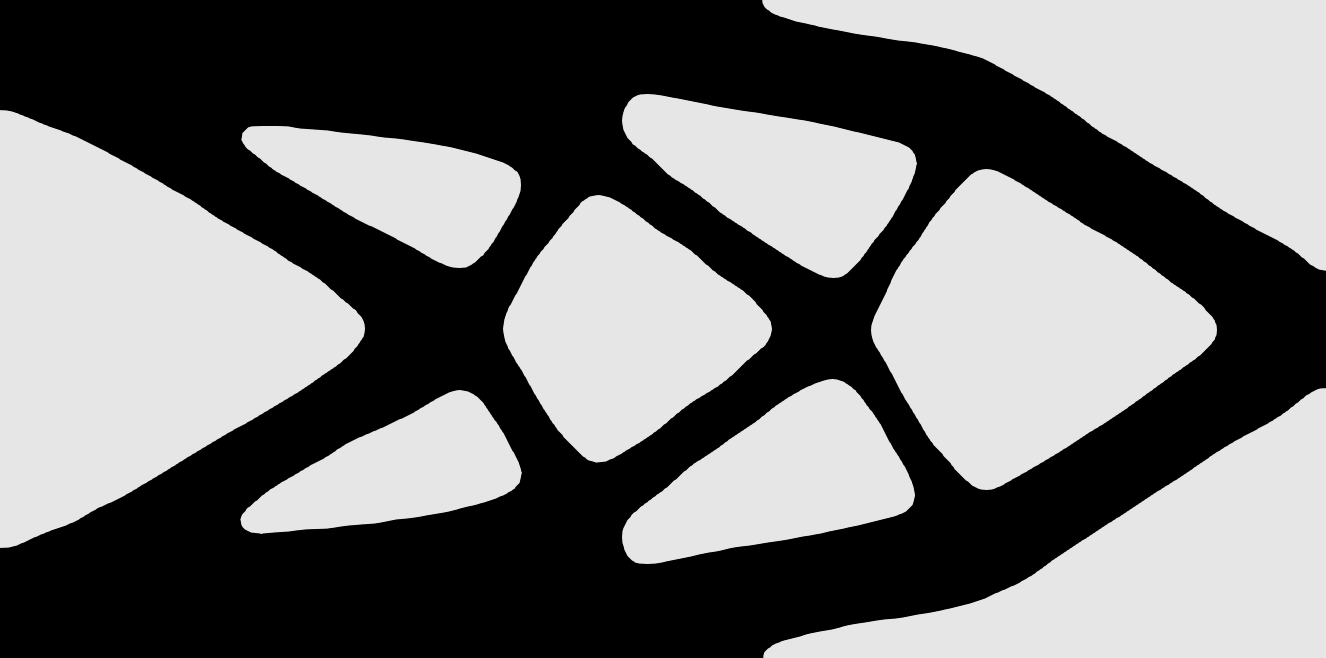
\includegraphics[width=0.48\linewidth]{compliance1.png}
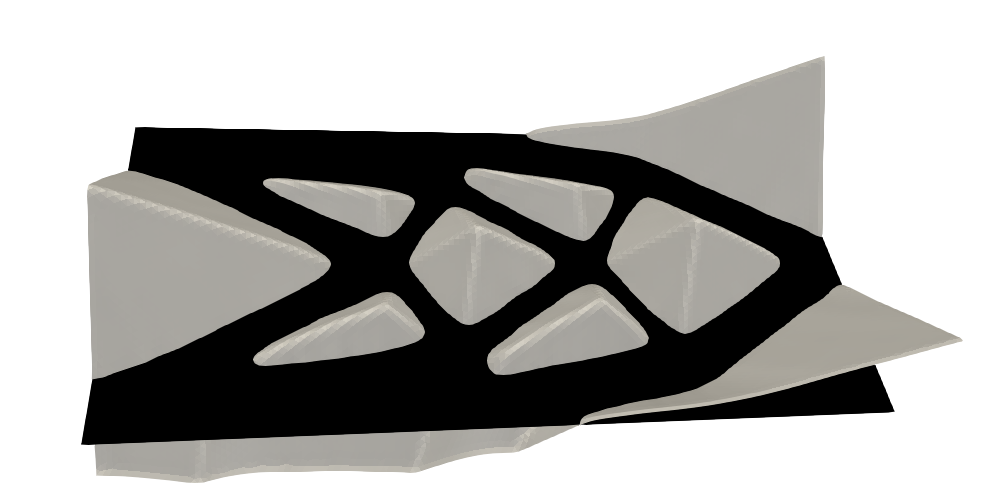
\includegraphics[width=0.85\linewidth]{compliance2.png}
\captionof{figure}{
	(top) Initial guess and optimized design.
	(bottom) The level set function approximates the distance function.
}
\label{fig:compli2D}
\end{center}

$\mathcal{D} = (0, 2)\times(0, 1)\times(0, 1)$

$\{x=0, 0<y<1, 0<z<1\}$

$\{x=1, 0.4<y<0.6, 0.4<z<0.6\}$

$g = (0, 0, -4)$
\begin{center}
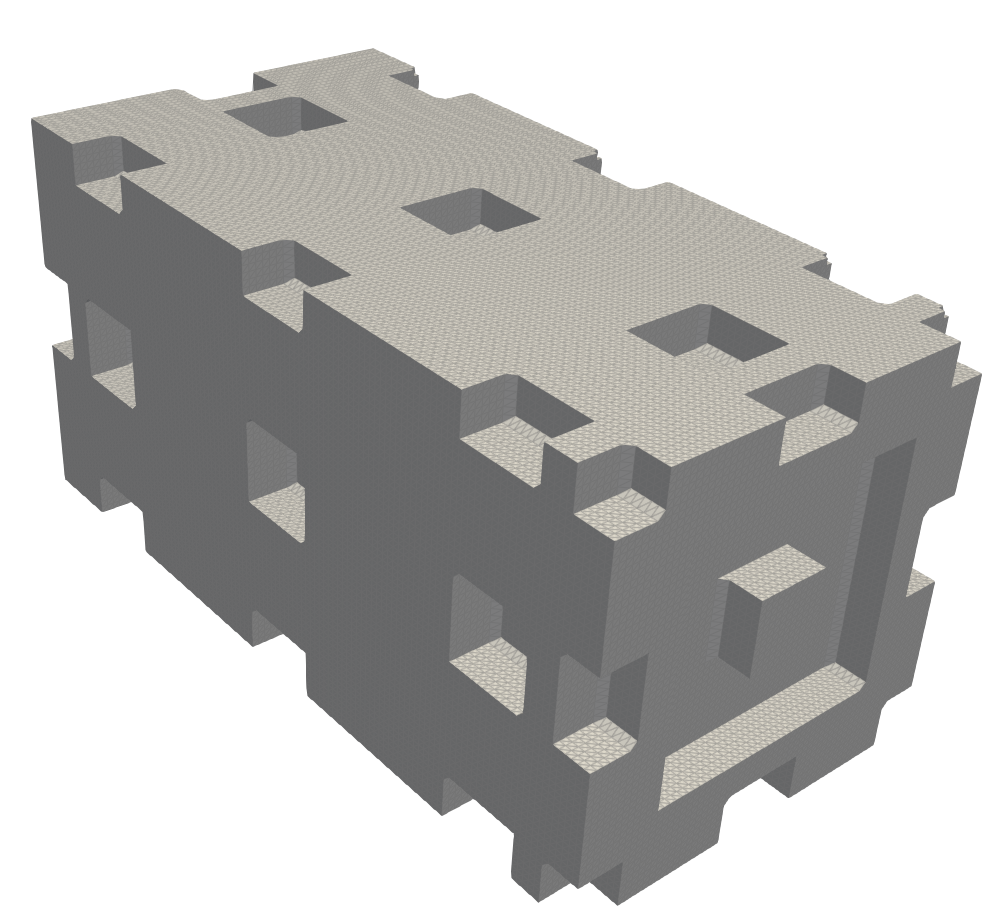
\includegraphics[width=0.48\linewidth]{compli3D_0.png}
\hfill
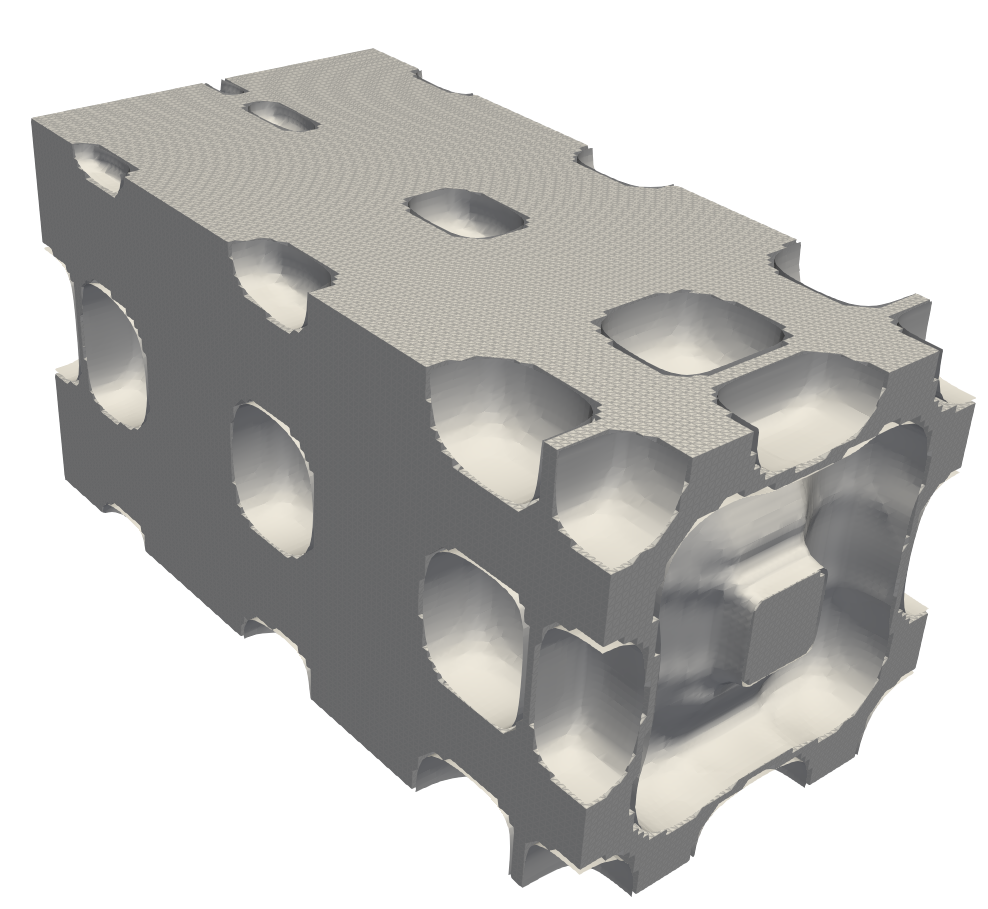
\includegraphics[width=0.48\linewidth]{compli3D_1.png}
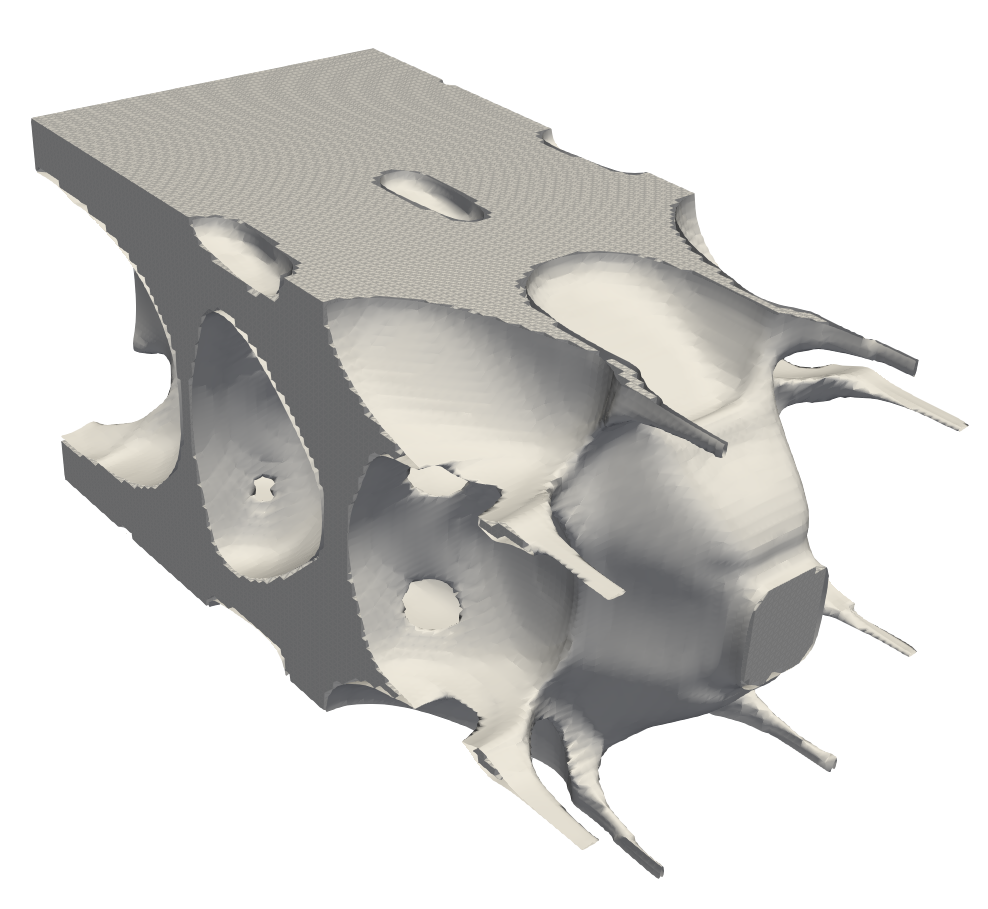
\includegraphics[width=0.48\linewidth]{compli3D_2.png}
\hfill
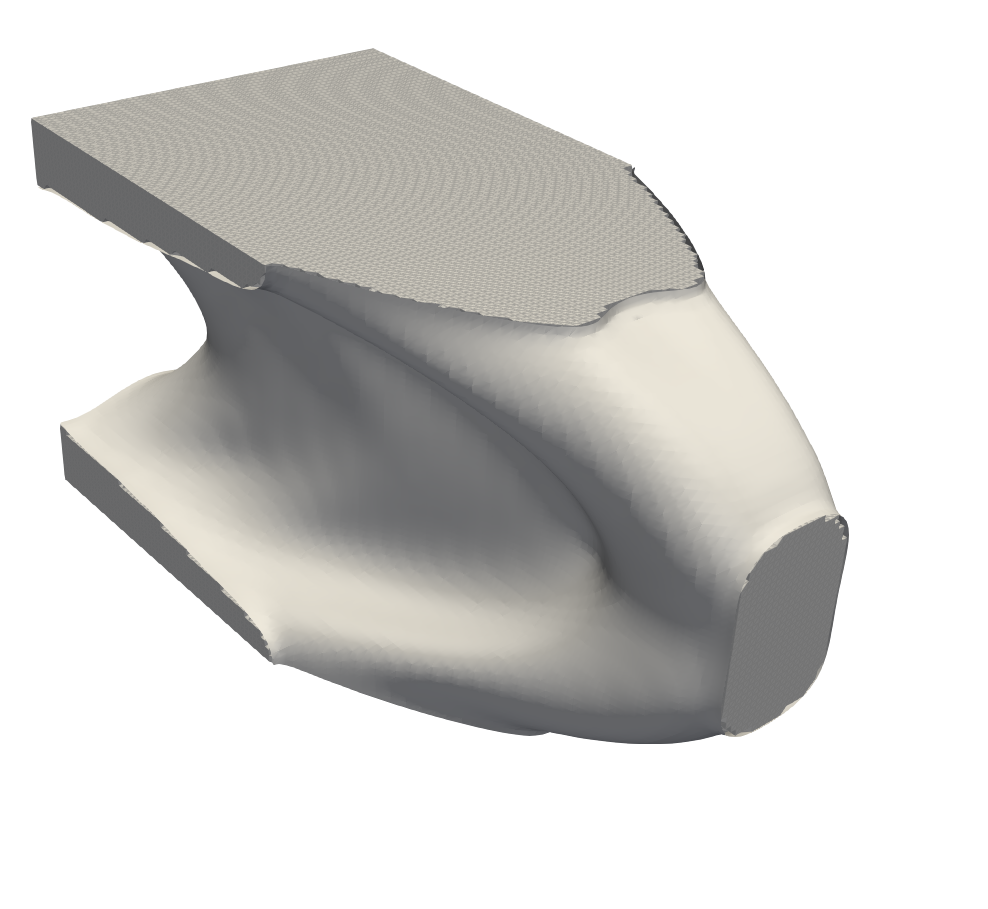
\includegraphics[width=0.48\linewidth]{compli3D_3.png}
\captionof{figure}{
	Some iterations of the three-dimensional
	cantilever.
}
\label{fig:compli3D}
\end{center}

\textbf{Multiple load cases.}
\begin{center}
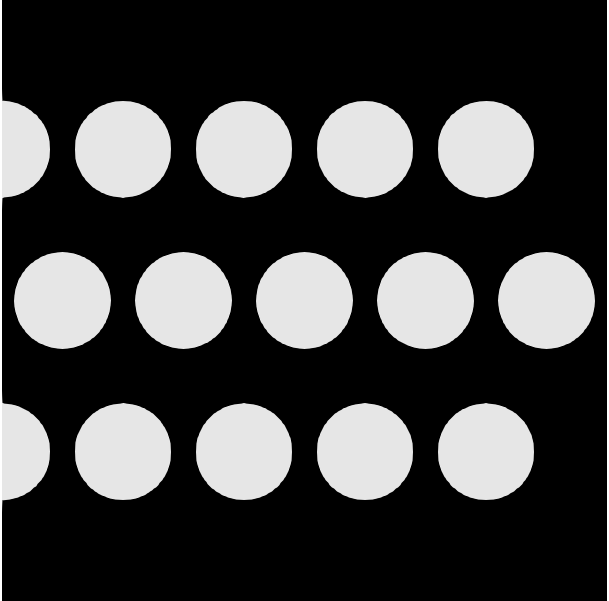
\includegraphics[width=0.48\linewidth]{compliplus1_0.png}
\hfill
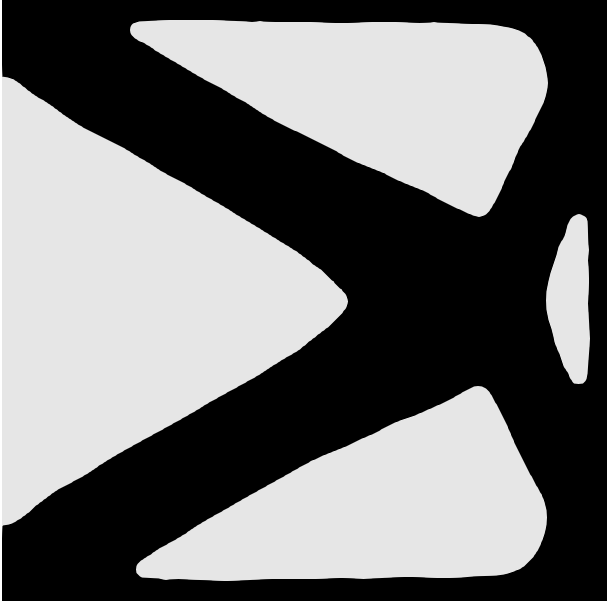
\includegraphics[width=0.48\linewidth]{compliplus1_1.png}

\vspace{0.3cm}

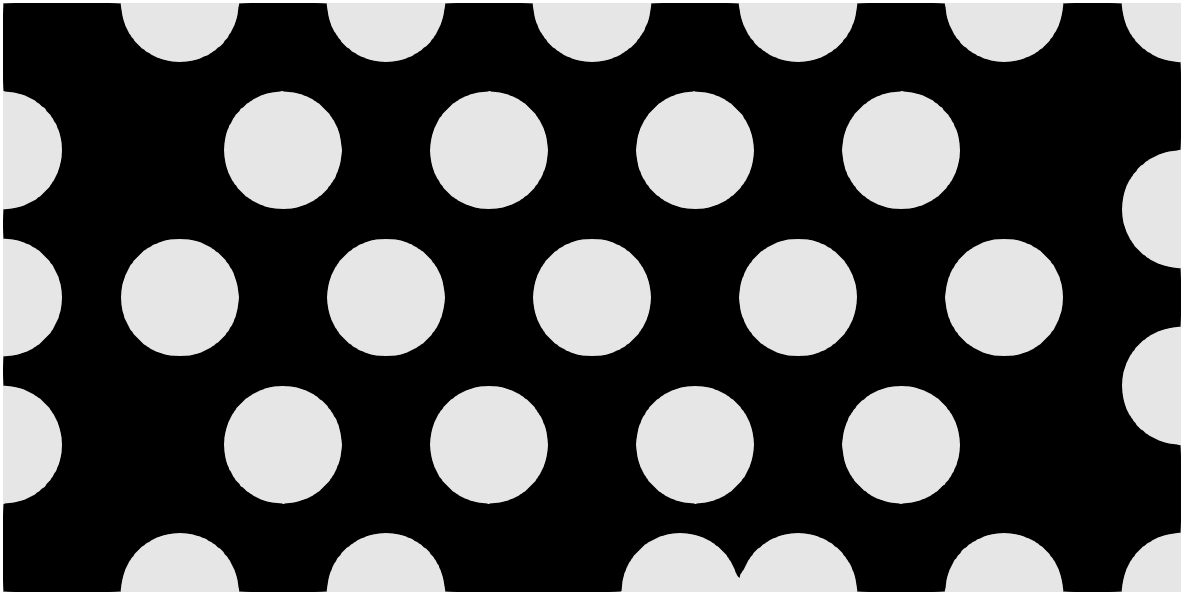
\includegraphics[width=0.48\linewidth]{compliplus2_0.png}
\hfill
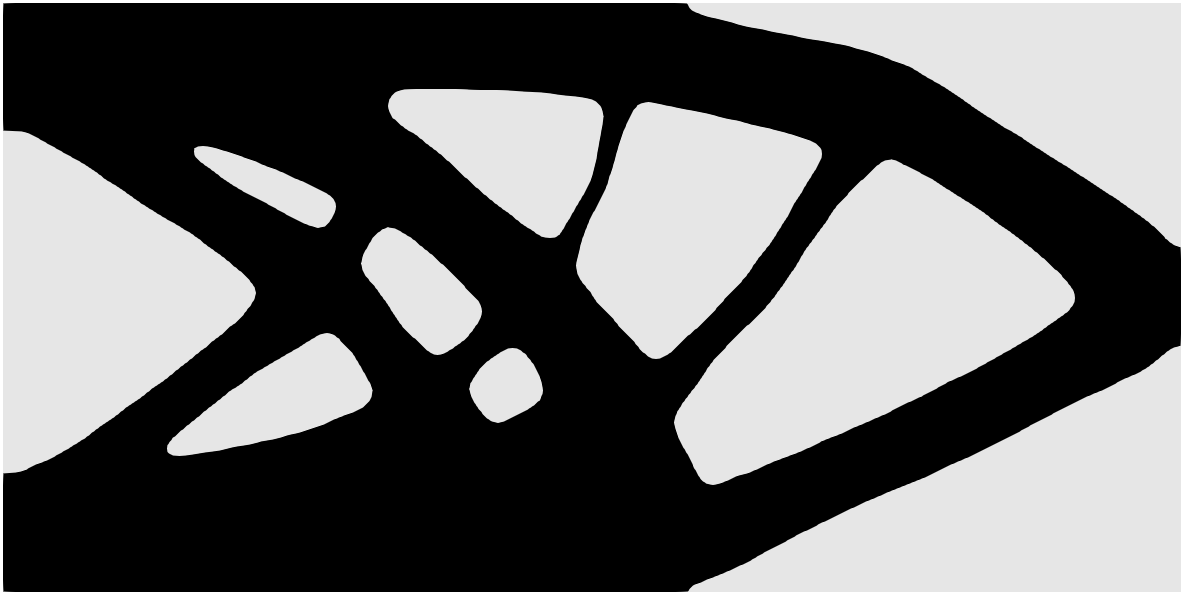
\includegraphics[width=0.48\linewidth]{compliplus2_1.png}
\captionof{figure}{
	(Top) (Bottom)
}
\label{fig:compliplus}
\end{center}



\subsection{Heat Conduction}

%%%%%%%%%%%%%%%%%%%%%%%
\subsection{Performance investigation}
%%%%%%%%%%%%%%%%%%%%%%%

Here we should discuss some performance data of the code. Show that the code is extremely fast in 2D. Show what size of 3D problems we can consider using a server (also large amount of sources).
Also maybe show weak scalabilty tests for parallel computing, as in \cite{Jia2024}.




%%%%%%%%%%%%%%%%%%%%%%%
\section{Conclusion}
%%%%%%%%%%%%%%%%%%%%%%%

In the conclusion we discuss possible future extensions of this toolbox. Here are some ideas.
\begin{itemize}
\item higher-order tensors such as biLaplacian problems
\item Boundary terms for surface problems.
\item automatic differentiation?
\end{itemize}    


\end{multicols} 

\bibliographystyle{plain}
\bibliography{distributed}


\end{document}

